\documentclass{standalone}
\usepackage{graphicx}	
\usepackage{amssymb, amsmath, amsthm}
\usepackage{color}

\usepackage{tikz}
\usetikzlibrary{arrows.meta, math}

\definecolor{light}{RGB}{220, 188, 188}
\definecolor{mid}{RGB}{185, 124, 124}
\definecolor{dark}{RGB}{143, 39, 39}
\definecolor{highlight}{RGB}{180, 31, 180}
\definecolor{lightteal}{RGB}{107, 142, 142}
\definecolor{midteal}{RGB}{72, 117, 117}
\definecolor{darkteal}{RGB}{29, 79, 79}
\definecolor{gray10}{gray}{0.1}
\definecolor{gray20}{gray}{0.2}
\definecolor{gray30}{gray}{0.3}
\definecolor{gray40}{gray}{0.4}
\definecolor{gray60}{gray}{0.6}
\definecolor{gray70}{gray}{0.7}
\definecolor{gray80}{gray}{0.8}
\definecolor{gray90}{gray}{0.9}
\definecolor{gray95}{gray}{0.95}

\tikzmath{
  % Horizontal position of center of circumcircle
  function circumcirclex(\xa, \ya, \xb, \yb, \xc, \yc) {
    return 0.5 * (  (\yc - \ya) * (\yc - \yb) * (\yb - \ya)
                  + (\xc * \xc - \xb * \xb) * (\yb - \ya)
                  - (\xb * \xb - \xa * \xa) * (\yc - \yb) ) / 
           ( (\xc - \xb) * (\yb - \ya) - (\xb - \xa) * (\yc - \yb));
  };
  % Vertical position of center of circumcircle
  function circumcircley(\xv, \xa, \ya, \xb, \yb, \xc, \yc) {
    return - (\xb - \xa) / (\yb - \ya) * (\xv - 0.5 * (\xa + \xb)) + 0.5 * (\ya + \yb);
  };
  % Slope of perpendicular bisector between two points
  function mperbi(\xa, \ya, \xb, \yb) {
    \m = ( \yb - \ya ) / ( \xb - \xa );
    return - 1 / \m;
  };
}

\begin{document}

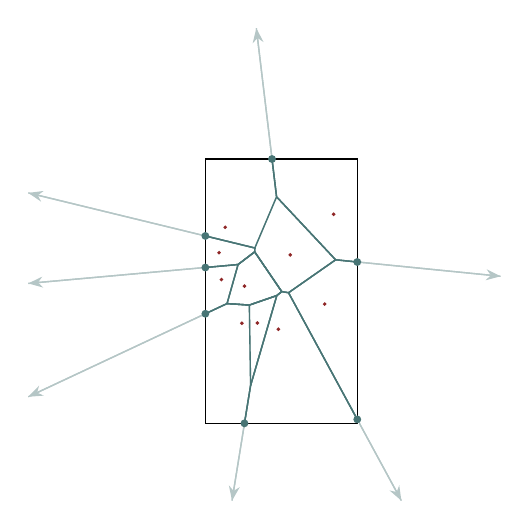
\begin{tikzpicture}
  \draw[white] (-3, -3) rectangle (3, 3);
  \clip (-3, -3) rectangle (3, 3);
  
  % Face 7
  \draw[lightteal!50!white, line width=0.5] (-0.475, -0.497)
    \foreach \x/\y in {-0.192/-0.516, 0.157/-0.395, 0.220/-0.345, -0.124/0.160, -0.335/-0.001, -0.335/-0.001} {
      -- (\x, \y)
  }; 

  % Face 3
  \draw[->, >=Stealth, lightteal!50!white, line width=0.5] (-0.412, -3.000)
    \foreach \x/\y in {-0.176/-1.538, -0.192/-0.516, -0.475/-0.497, -3.000/-1.681} {
      -- (\x, \y)
  };  

  % Face 9
  \draw[->, >=Stealth, lightteal!50!white, line width=0.5] (1.739, -3.000)
    \foreach \x/\y in {0.306/-0.359, 0.220/-0.345, 0.157/-0.395, -0.176/-1.538, -0.412/-3.000 } {
      -- (\x, \y)
  };  

  % Face 4
  \draw[->, >=Stealth, lightteal!50!white, line width=0.5] (3.000, -0.150)
    \foreach \x/\y in {0.904/0.059, 0.306/-0.359, 1.739/-3.000} {
      -- (\x, \y)
  }; 

  % Face 5
   \draw[->, >=Stealth, lightteal!50!white, line width=0.5] (-0.103, 3.000)
    \foreach \x/\y in {0.154/0.859, 0.904/0.059, 3.000/-0.150} {
      -- (\x, \y)
  }; 

  % Face 1
  \draw[->, >=Stealth, lightteal!50!white, line width=0.5] (-3.000, 0.909)
    \foreach \x/\y in {-0.122/0.209, 0.154/0.859, -0.103/3.000 } {
      -- (\x, \y)
  }; 


  % Face 6 
  \draw[->, >=Stealth, lightteal!50!white, line width=0.5] (-3.000, -0.241)
    \foreach \x/\y in {-0.335/-0.001, -0.124/0.160, -0.122/0.209, -3.000/0.909} {
      -- (\x, \y)
  }; 

  % Face 2 
  \draw[->, >=Stealth, lightteal!50!white, line width=0.5] (-3.000, -1.681)
    \foreach \x/\y in {-0.475/-0.497, -0.335/-0.001, -3.000/-0.241} {
      -- (\x, \y)
  }; 


  % Face 8
  \draw[lightteal!50!white, line width=0.5] (-0.122, 0.209)
    \foreach \x/\y in {-0.124/0.160, 0.220/-0.345, 0.306/-0.359, 0.904/0.059, 0.154/0.859, 0.154/0.859} {
      -- (\x, \y)
  }; 

  % Face 10
  \draw[lightteal!50!white, line width=0.5] (-0.176, -1.538)
    \foreach \x/\y in {0.157/-0.395, -0.192/-0.516, -0.192/-0.516} {
      -- (\x, \y)
  };
  
  \foreach \x/\y in {-0.498/0.472, -0.546/-0.192, -0.286/-0.747, 
                     0.765/-0.503, 0.878/0.637, -0.577/0.149, 
                     -0.254/-0.275, 0.328/0.122, 0.177/-0.822, -0.090/-0.744} {
    \fill[dark] (\x, \y) circle (0.025);
  }
  
  \draw[midteal, line width=0.5] (-0.475, -0.497)
    \foreach \x/\y in {-0.475/-0.497, -0.192/-0.516, 
                       0.157/-0.395, 0.220/-0.345, -0.124/0.160, 
                      -0.335/-0.001, -0.475/-0.497} {
      -- (\x, \y)
  };
  
  % Face 7
  \draw[midteal, line width=0.5] (-0.475, -0.497)
    \foreach \x/\y in {-0.192/-0.516, 0.157/-0.395, 0.220/-0.345, -0.124/0.160, -0.335/-0.001, -0.335/-0.001} {
      -- (\x, \y)
  }; 

  % Face 3
  \draw[midteal, line width=0.5] (-0.254, -2.018)
    \foreach \x/\y in {-0.176/-1.538, -0.192/-0.516, -0.475/-0.497, -0.750/-0.626} {
      -- (\x, \y)
  };  

  % Face 9
  \draw[midteal, line width=0.5] (1.179, -1.968)
    \foreach \x/\y in {0.306/-0.359, 0.220/-0.345, 0.157/-0.395, -0.176/-1.538, -0.254/-2.018 } {
      -- (\x, \y)
  };  

  % Face 4
  \draw[midteal, line width=0.5] (1.179, 0.031)
    \foreach \x/\y in {0.904/0.059, 0.306/-0.359, 1.179/-1.968} {
      -- (\x, \y)
  }; 

  % Face 5
   \draw[midteal, line width=0.5] (0.096, 1.339)
    \foreach \x/\y in {0.154/0.859, 0.904/0.059, 1.179/0.031} {
      -- (\x, \y)
  }; 

  % Face 1
  \draw[midteal, line width=0.5] (-0.750, 0.362)
    \foreach \x/\y in { -0.122/0.209, 0.154/0.859, 0.096/1.339 } {
      -- (\x, \y)
  }; 

  % Face 6 
  \draw[midteal, line width=0.5] (-0.750, -0.039)
    \foreach \x/\y in {-0.335/-0.001, -0.124/0.160, -0.122/0.209, -0.750/0.362} {
      -- (\x, \y)
  }; 

  % Face 2 
  \draw[midteal, line width=0.5] (-0.750, -0.626)
    \foreach \x/\y in {-0.475/-0.497, -0.335/-0.001, -0.750/-0.039} {
      -- (\x, \y)
  }; 

  % Face 8
  \draw[midteal, line width=0.5] (-0.122, 0.209)
    \foreach \x/\y in {-0.124/0.160, 0.220/-0.345, 0.306/-0.359, 0.904/0.059, 0.154/0.859, 0.154/0.859} {
      -- (\x, \y)
  }; 

  % Face 10
  \draw[midteal, line width=0.5] (-0.176, -1.538)
    \foreach \x/\y in {0.157/-0.395, -0.192/-0.516, -0.192/-0.516} {
      -- (\x, \y)
  }; 
  
  \draw[white, line width=1] (1.1793552, 1.339005) rectangle (-0.7503322, -2.017567);
  \draw[black, line width=0.5] (1.1793552, 1.339005) rectangle (-0.7503322, -2.017567);

  \fill[midteal] (-0.254, -2.018) circle (0.05);
  \fill[midteal] (1.179, -1.968) circle (0.05);
  \fill[midteal] (1.179, 0.031) circle (0.05);
  \fill[midteal] (0.096, 1.339) circle (0.05);
  \fill[midteal] (-0.750, 0.362) circle (0.05);
  \fill[midteal] (-0.750, -0.039) circle (0.05);
  \fill[midteal] (-0.750, -0.626) circle (0.05);

\end{tikzpicture}

\end{document}  